\documentclass{beamer}
%\documentclass[handout]{beamer}
%\setbeameroption{show notes}

% Think backwards: what do you want people to remember from your talk?
% Don’t say everything.
% Simplify.

\usecolortheme[named=blue]{structure}
\mode<presentation>
{
  \usetheme{Warsaw}
  \setbeamercovered{transparent}
}
\usepackage{listings}
%\lstset{basicstyle=\scriptsize}
\usepackage[english]{babel}
\usepackage[utf8]{inputenc}
\usepackage{amsmath}
\usepackage{graphicx}
\usepackage{fontenc}
\usepackage{tikz}

\title[{Nopol: Repairing Bugs in Conditional Expressions}]{Nopol:~Repairing~Bugs~in~Conditional~Expressions}
\author[Favio DeMarco]{Favio~DeMarco}
\institute[U.B.A. - INRIA]{Universidad de Buenos Aires - INRIA}
\date{\today}
\subject{Computational Sciences}

\begin{document}

  \frame
  {
\begin{quote}
    Take nothing on its looks; take everything on evidence. There's no better rule.
\end{quote}    
– Charles Dickens, ``Great Expectations.''
  }

\frame
  {
  \begin{center}
  
\includegraphics[width=7em]{logofcen}
  \end{center}
    \titlepage
  }

\begin{frame}[fragile]
\frametitle{What are conditional bugs?}
\begin{lstlisting}[escapeinside=\[\]]
[\textbf{boolean expression}] ? someValue : someOtherValue;
\end{lstlisting}

\begin{lstlisting}[escapeinside=\[\]]
if ([\textbf{boolean expression}]) {
...
\end{lstlisting}
\end{frame}
  
\begin{frame}[fragile]
\frametitle{What are conditional bugs?}
\framesubtitle{Commons Math - MathUtils class}
    
\begin{lstlisting}[escapeinside=\[\]]
public static int gcd(int u, int v) {
  if ([\textbf{u * v == 0}]) {
    return Math.abs(u) + Math.abs(v);
  }
...
\end{lstlisting}

\vspace{2em}

\centering What about \texttt{u=0x00110000} and  \texttt{v=0x01100000}?

\end{frame}

\begin{frame}
\frametitle{Problem}
\framesubtitle{How to find the bug?}
How do we know something is \textit{wrong}?
\end{frame}

\begin{frame}
\frametitle{Problem}
\framesubtitle{How to find the bug?}
Specification:
\begin{itemize}
 \item Model
 \item Contracts
 \item \textbf{Unit tests}
 \item ...
\end{itemize}
\end{frame}

 \begin{frame}[fragile]
    \frametitle{Case study}
      \framesubtitle{Commons Math}
At least one failing test:
      
      \begin{lstlisting}[escapeinside=\[\]]
assertEquals([\textbf{3 * (1$<<$15)}]
        , gcd(3 * (1<<20), 9 * (1<<15)));
	\end{lstlisting}
\end{frame}

\frame
{
    \frametitle{Algorithm}
    \framesubtitle{Trial and error}
  \begin{center}
  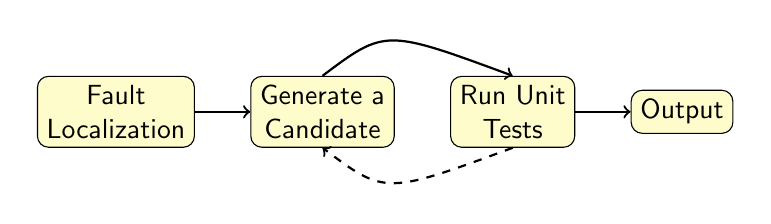
\begin{tikzpicture}[
  font=\sffamily,
  every matrix/.style={ampersand replacement=\&,column sep=2em,row sep=2em},
  box/.style={draw,rounded corners,fill=yellow!20},
  flow/.style={->, thick},
  fail/.style={->, thick, dashed},
  every node/.style={align=center}]
  
% Position the nodes using a matrix layout
\matrix{
      \node[box] (faultLocalization) {Fault \\ Localization};
      \& \node[box] (generateCandidate) {Generate a \\ Candidate};
      \& \node[box] (test) {Run Unit \\ Tests};
      \& \node[box] (output) {Output};
      \\
  };

% Draw the arrows between the nodes and label them.
\draw [flow] (faultLocalization) -- (generateCandidate);
\draw [flow] (generateCandidate.north) .. controls (up:3em) .. (test.north);
\draw [flow] (test) -- (output);
\draw [fail] (test.south) .. controls (down:3em) .. (generateCandidate.south);


% \draw [fail] (oracleInquisition.south) .. controls (down:.5em) and (left:8em) .. (oracleInquisition.west);
% \draw [fail] (collectionOfTestExecutionData) .. controls (down:2em) and (left:9em) .. (oracleInquisition.west);
% \draw [fail] (smtSolving.north) .. controls (down:2em) and (left:10em) .. (oracleInquisition.west);
\end{tikzpicture}

  \end{center}

\texttt{statements =} \textit{statement ranking}\texttt{()}

\texttt{do}

$\rightarrow$ \texttt{statement = statements.pop()}

$\rightarrow$ \textit{generate a candidate and apply it}\texttt{(statement)}

\texttt{while} \textit{it doesn't pass all tests} \texttt{\& statements $\neq \varnothing$}

\texttt{return} \textit{patch or $\varnothing$}
}


 \begin{frame}[fragile]
    \frametitle{Statement ranking}
      \framesubtitle{GZoltar - Ochiai coefficient}
Suspiciousness $s_j$ of a statement $j$:
\begin{equation*}
 s_j=\dfrac{ee_j}{\sqrt{(ee_j + ne_j ) \times (ee_j + en_j )}}
\end{equation*}
\begin{itemize}
 \item $ee_j$: number of \textbf{failing} test cases \textbf{executing} statement $j$ 
 \item $ne_j$: number of \textbf{failing} test cases \textbf{not executing} statement $j$
 \item $en_j$: number of \textbf{successful} tests \textbf{executing} statement $j$
\end{itemize}
\end{frame}


 \begin{frame}[fragile]
    \frametitle{Statement ranking}
      \framesubtitle{GZoltar - Ochiai coefficient}
\begin{verbatim}
MathUtils:413 Suspiciousness 0.23570226039551587
MathUtils:431 Suspiciousness 0.1543033499620919
\end{verbatim}
...
\begin{verbatim}
MathUtils:460 Suspiciousness 0.11322770341445956
MathUtils:412 Suspiciousness 0.11180339887498948
\end{verbatim}
\end{frame}

\frame
{
  \begin{center}
  \begin{tikzpicture}[
  font=\sffamily,
  every matrix/.style={ampersand replacement=\&,column sep=2em,row sep=2em},
  box/.style={rounded corners,fill=gray,path fading=south},
  shadedbox/.style={rounded corners,fill=black!90},
  flow/.style={->, very thick},
  fail/.style={->, thick, dashed},
  every node/.style={align=center}]
  
% Position the nodes using a matrix layout
\matrix{
    \node[shadedbox] (faultLocalization) {Fault \\ Localization};
      \& \node[box] (oracleInquisition) {Oracle \\ Inquisition};
      \& \node[box] (collectionOfTestExecutionData) {Collection \\ of Test Execution \\ Data};
      \& \\

    \node[shadedbox] (sourceCodeSynthesis) {Source \\ Code \\ Synthesis};
      \& \node[box] (smtSolving) {SMT \\ Solving};
      \& \node[box] (constraintsGeneration) {Constraints \\ Generation}; \\
  };

% Draw the arrows between the nodes and label them.
\draw [flow] (faultLocalization) -- (oracleInquisition);
\draw [flow] (oracleInquisition) -- (collectionOfTestExecutionData);
\draw [flow] (collectionOfTestExecutionData) -- (constraintsGeneration);
\draw [flow] (constraintsGeneration) -- (smtSolving);
\draw [flow] (smtSolving) -- (sourceCodeSynthesis);

\draw [fail] (oracleInquisition.south) .. controls (down:.5em) and (left:8em) .. (oracleInquisition.west);
\draw [fail] (collectionOfTestExecutionData) .. controls (down:2em) and (left:9em) .. (oracleInquisition.west);
\draw [fail] (smtSolving.north) .. controls (down:2em) and (left:10em) .. (oracleInquisition.west);
\end{tikzpicture}

  \end{center}
}

  \frame
  {
    \frametitle{Problems}
\begin{itemize}
\item Can't automate the testing process.
\item It's not easy to find candidates.
\end{itemize}    
  }

  \frame
  {
    \frametitle{Problems}
    \framesubtitle{Test quality}
   \begin{quote}
    Quality is free, but only to those who are willing to pay heavily for it.
   \end{quote}
    Tom DeMarco, Peopleware   
  }
  
  \frame
  {
    \frametitle{Limitations}
    \framesubtitle{Test quality}
\begin{itemize}
\item Only 1 set of input values.
\item Branch coverage.
\item A \textit{removed} precondition can generate an infinite loop.
\item Tests that exercise both branches.
\item Generates \textit{a} fix not \textbf{THE} fix.
\end{itemize}        
  }

  \frame
  {  
    \frametitle{Contributions}
      \framesubtitle{Process}
\begin{itemize}
\item Statement ranking (GZoltar)  $\rightarrow$
\item Ad hoc code manipulation and values capturing $\rightarrow$
\item Repair Constraint  $\rightarrow$
\item Program Synthesis (OGCBPS\footnote{Oracle-Guided Component-Based Program Synthesis} -paper-)
\end{itemize}
}


  \frame
  {
    \frametitle{Experimental methodology}
    Seeded and wild bugs.
  }
  
  \frame
  {
    \frametitle{Evaluation / Validation}
    Generated patches vs. reality.
  }
  
  \frame
  {
    \frametitle{Perspectives}
    
  }
  
  \frame
  {
    \frametitle{Conclusion}
    
  }

  \frame
  {
    \frametitle{Contribution}
    
  }
  
 \begin{frame}[fragile]
    \frametitle{Case study}
      \framesubtitle{Commons Math - MathUtils class}
\begin{lstlisting}[escapeinside=\[\]]
411: public static int gcd(int u, int v) {
412:   if ([\textbf{u * v == 0}]) {
413:     return (Math.abs(u) + Math.abs(v));
414:   }
...
\end{lstlisting}
\end{frame}

 \begin{frame}[fragile]
    \frametitle{Case study}
      \framesubtitle{Commons Math}
        \begin{lstlisting}[escapeinside=\[\]]
assertEquals([\textbf{3 * (1$<<$15)}]
        , gcd(3 * (1<<20), 9 * (1<<15)));
	\end{lstlisting}
\end{frame}

 \begin{frame}[fragile]
    \frametitle{Case study}
      \framesubtitle{Statement ranking (GZoltar)}
\begin{verbatim}
MathUtils:413 Suspiciousness 0.23570226039551587
MathUtils:431 Suspiciousness 0.1543033499620919
\end{verbatim}
...
\begin{verbatim}
MathUtils:460 Suspiciousness 0.11322770341445956
MathUtils:412 Suspiciousness 0.11180339887498948
\end{verbatim}
\end{frame}

 \begin{frame}[fragile]
    \frametitle{Case study}
      \framesubtitle{Ad hoc code manipulation and values capturing (OGCBPS -paper-)}
\begin{lstlisting}[escapeinside=\[\]]
411: public static int gcd(int u, int v) {
412:   if ([\textbf{true}]) {
413:     return (Math.abs(u) + Math.abs(v));
414:   }
...
\end{lstlisting}
\end{frame}

 \begin{frame}[fragile]
    \frametitle{What are conditional bugs?}
    \framesubtitle{Commons Math - MathUtils class}
        \begin{lstlisting}[escapeinside=\[\]]
public static int gcd(int u, int v) {
    if ([\textbf{(u == 0) $||$ (v == 0)}]) {
        return (Math.abs(u) + Math.abs(v));
    }
    // ...
}
	\end{lstlisting}
\end{frame}

\end{document}
